\section{\hologo{MiKTeX}}
\label{sec:mik}

\begin{widepar}
  \hologo{MiKTeX} 发行版的特点在于仅安装用户需要的宏包,节省了磁盘空间占用,但在部分实现细节上与 \hologo{TeX}\,Live 有所出入。该发行版支持 Windows、Linux 和 macOS。
\end{widepar}

\subsection{前提条件}

一台正常访问校园网的设备,详见 \ref{subsec:device}。

\subsection{下载安装程序}

\hologo{MiKTeX} 为 Windows 和 macOS 提供了独立的安装包\sidenote{为什么没有 Linux 呢,点击下面空降链接就知道了},可以点击下方超链接获取。由于安装程序版本在不断更新,链接失效时请前往 \href{https://mirrors.nju.edu.cn/download/TeX%20%E6%8E%92%E7%89%88%E7%B3%BB%E7%BB%9F}{TeX 排版系统下载页}。

\begin{itemize}
  \item \href{https://mirrors.nju.edu.cn/CTAN/systems/win32/miktex/setup/windows-x64/basic-miktex-21.12-x64.exe}{\faFile*[regular] Windows 版安装包(21.12)}
  \item \href{https://mirrors.nju.edu.cn/CTAN/systems/win32/miktex/setup/darwin-x86_64/miktex-22.1-darwin-x86_64.dmg}{\faFile*[regular] macOS 版安装包(22.1)}
\end{itemize}

下载好后,空降链接:
\hyperref[subsec:mik-win-mac]{\faWindows{}}\,
\hyperref[subsec:mik-linux]{\faLinux{}}\,
\hyperref[subsec:mik-win-mac]{\faApple{}}

\subsection{Windows}
\label{subsec:mik-win}

点击运行安装程序,如图~\ref{fig:install-mik-win}所示。

\begin{figure}[htbp]
  \caption{Windows 系统下 \hologo{MiKTeX} 的安装界面。}
  \label{fig:install-mik-win}
  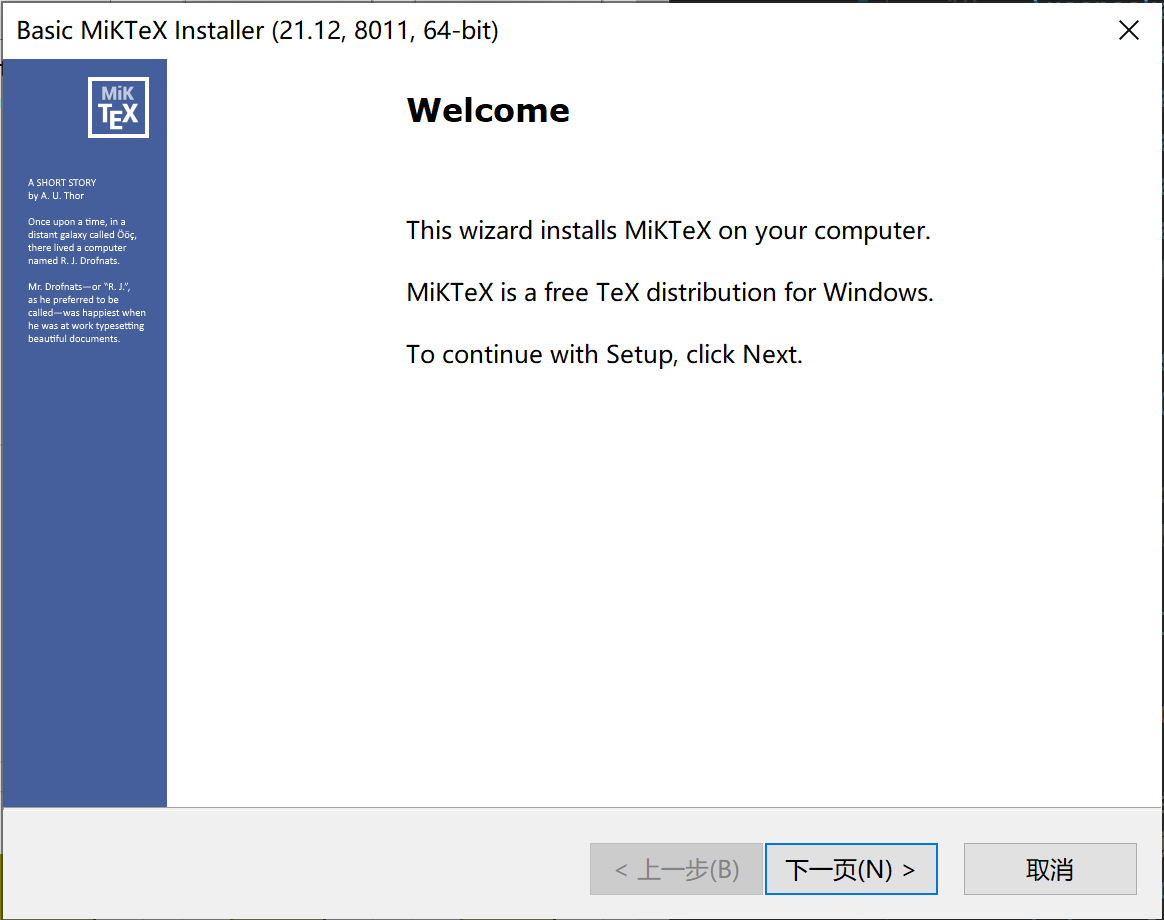
\includegraphics[width=0.7\textwidth]{install-mik-win}
\end{figure}

接下来,按上方显示的页面标题,可分为如下步骤:

\begin{description}
  \item[Welcome] 下一页 >
  \item[Copying Conditions] 勾选同意,下一页 >
  \item[Installation Scope] 保持默认设置\sidenote{为当前用户安装即可},下一页 >
  \item[Installation Directory] 保持默认设置\sidenote{如果 Windows 用户文件夹名称包含中文,可能会引发问题,见 \ref{subsec:device}},下一页 >
  \item[Settings] 第二个选项修改为 Yes\sidenote{一般让 \hologo{MiKTeX} 自动安装缺失的宏包,不然默认设置每次都会弹出对话框},下一页 >
  \item[Review] Start >
\end{description}

等待安装完成,就可以在开始菜单中找到 MiKTeX Console 应用程序。首次使用前需要打开此程序进行初始设置。如图~\ref{fig:miktex-console-win} 所示。要处理两个问题:
\begin{enumerate}
  \item 点击 PATH 问题的“立即修复”按钮,以添加系统环境变量。
  \item 从左侧栏切换到“更新”选项卡,点击“检查更新”按钮,待列表刷新后,点击“立即更新”按钮。
\end{enumerate}

\begin{figure}[htbp]
  \caption{首次在 Windows 打开 MiKTeX Console 显示的界面,此前出现的警告请先点击 OK 忽略。}
  \label{fig:miktex-console-win}
  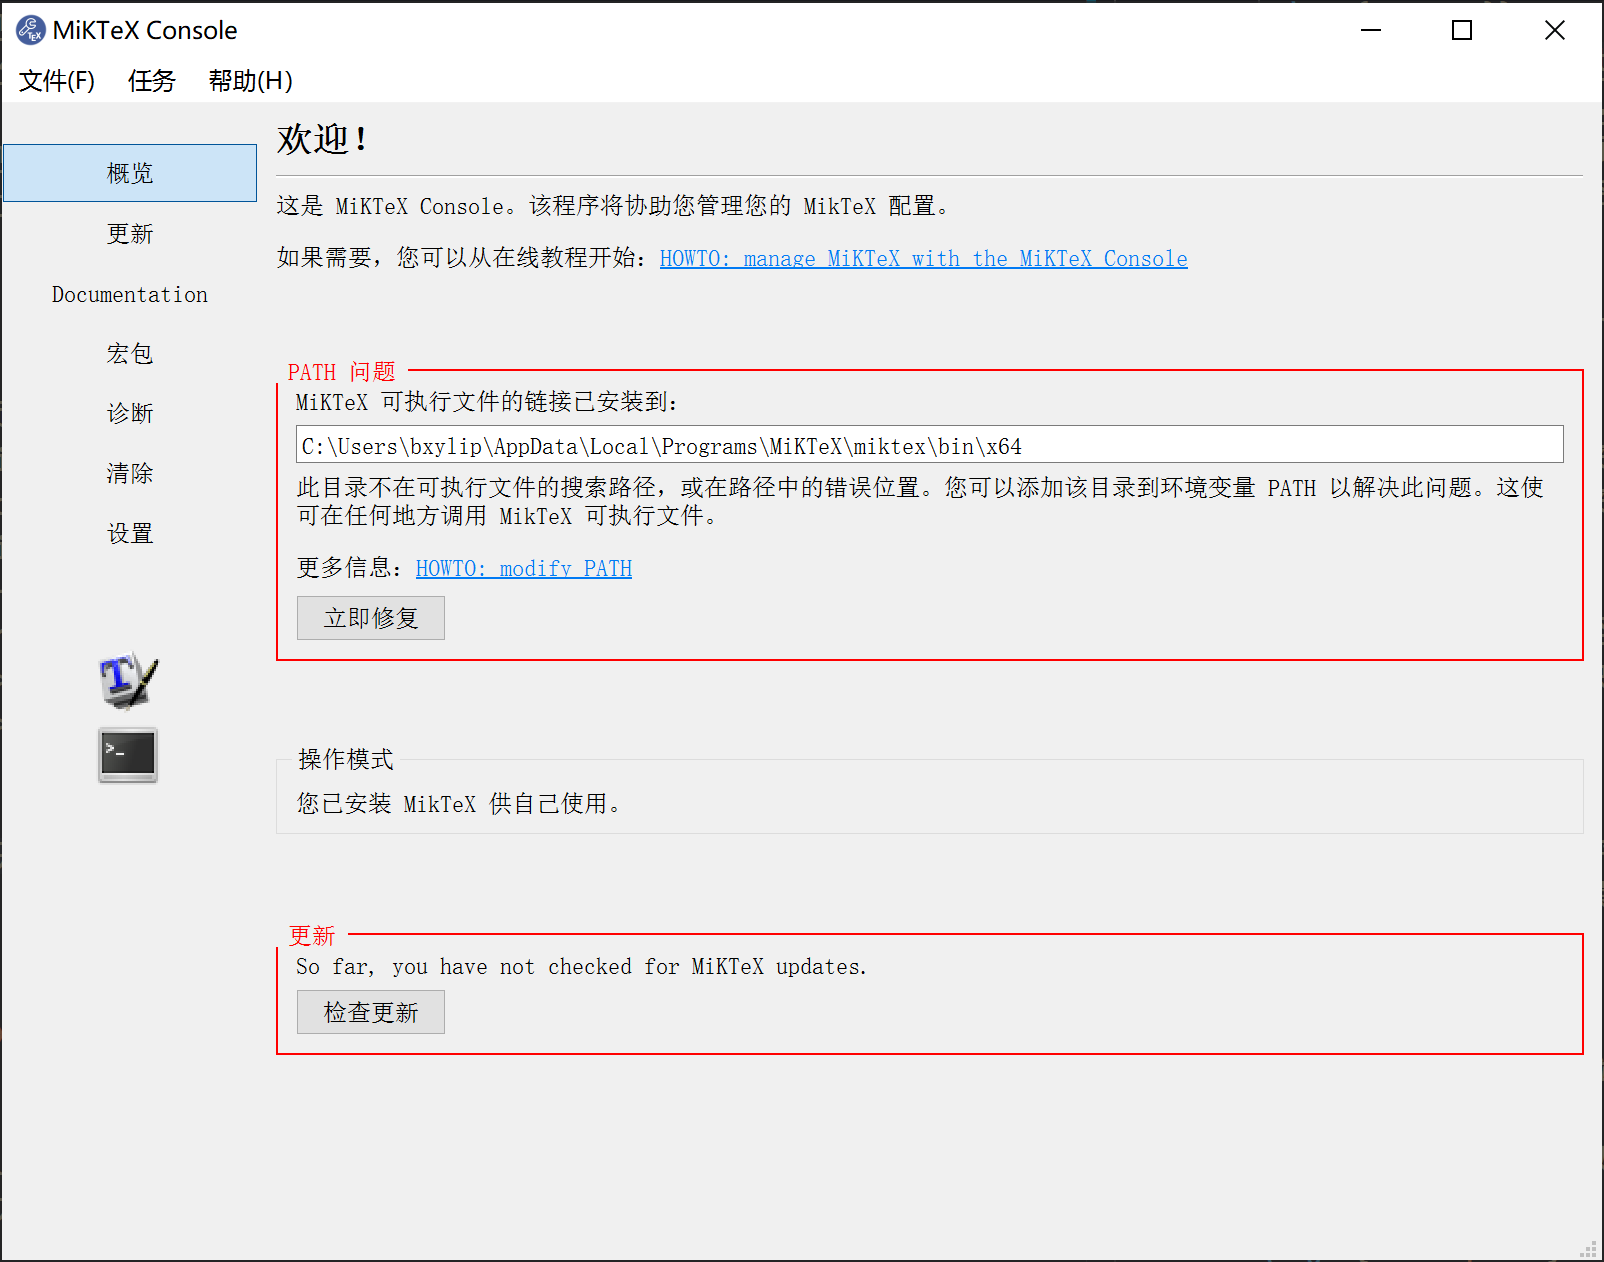
\includegraphics[width=0.8\textwidth]{miktex-console-win}
\end{figure}

在这个时间里,我们还要下载并安装 Strawberry Perl 程序。\sidenote{Perl 为 \texttt{latexmk} 脚本的依赖项,只有 Windows 系统下需要单独安装。这里推荐 Strawberry Perl。}

\begin{itemize}
  \item \href{https://strawberryperl.com/}{\faExternalLink* 官网下载,一般选 64bit 版}
\end{itemize}

无需更改任何选项,以默认设置安装即可。另一边,更新完成后可以关闭 MiKTeX Console 应用程序,接着阅读 \ref{sec:hw}。

\subsection{macOS}
\label{subsec:mik-mac}

\begin{widepar}
打开安装器,如图~\ref{fig:install-mik-mac} 所示,将 MiKTeX Console 拖动到到应用文件夹即可。
\end{widepar}

\begin{figure}[htbp]
  \caption{跟其他 macOS 应用程序安装器长得一样。}
  \label{fig:install-mik-mac}
  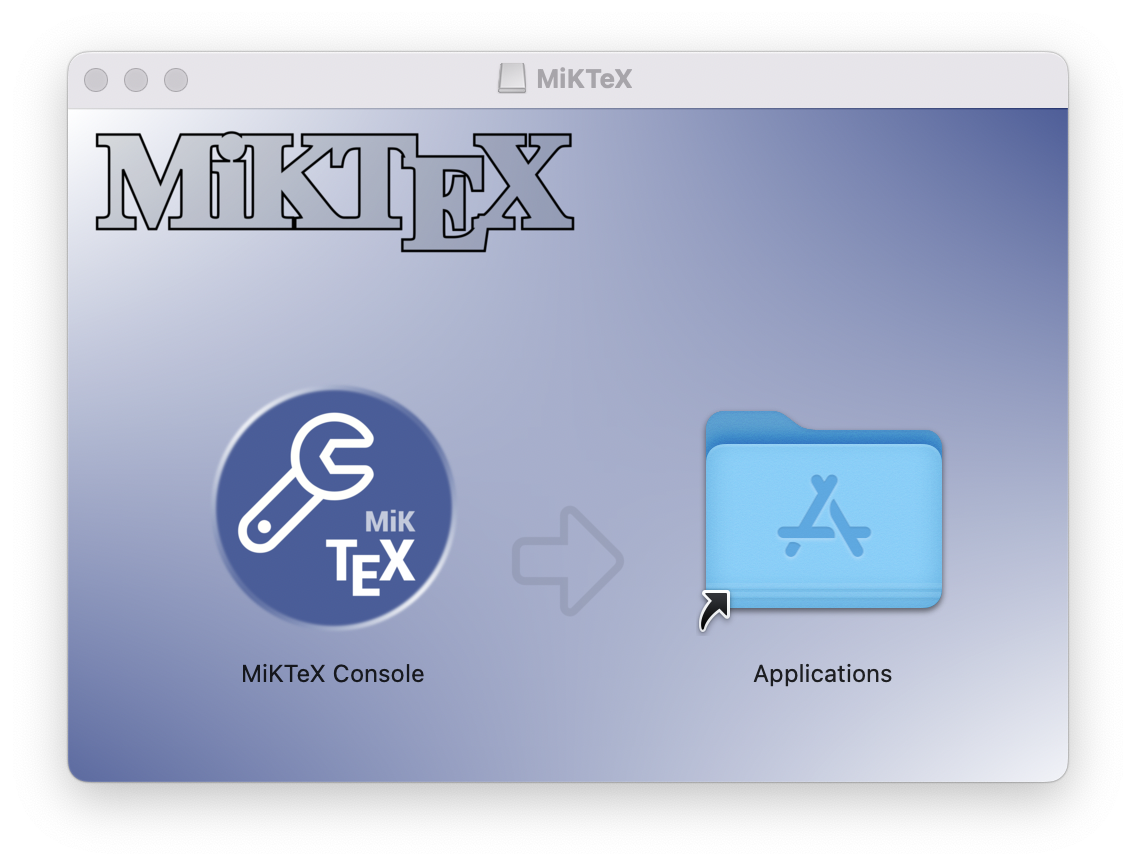
\includegraphics[width=0.5\textwidth]{install-mik-mac.png}
\end{figure}

接下来需要打开 MiKTeX Console 应用程序进行初始设置。首先需要完成安装向导,推荐第一项,即仅供个人使用。

\begin{figure}[htbp]
  \caption{首次在 macOS 打开 MiKTeX Console 显示的界面。}
  \label{fig:miktex-console-mac}
  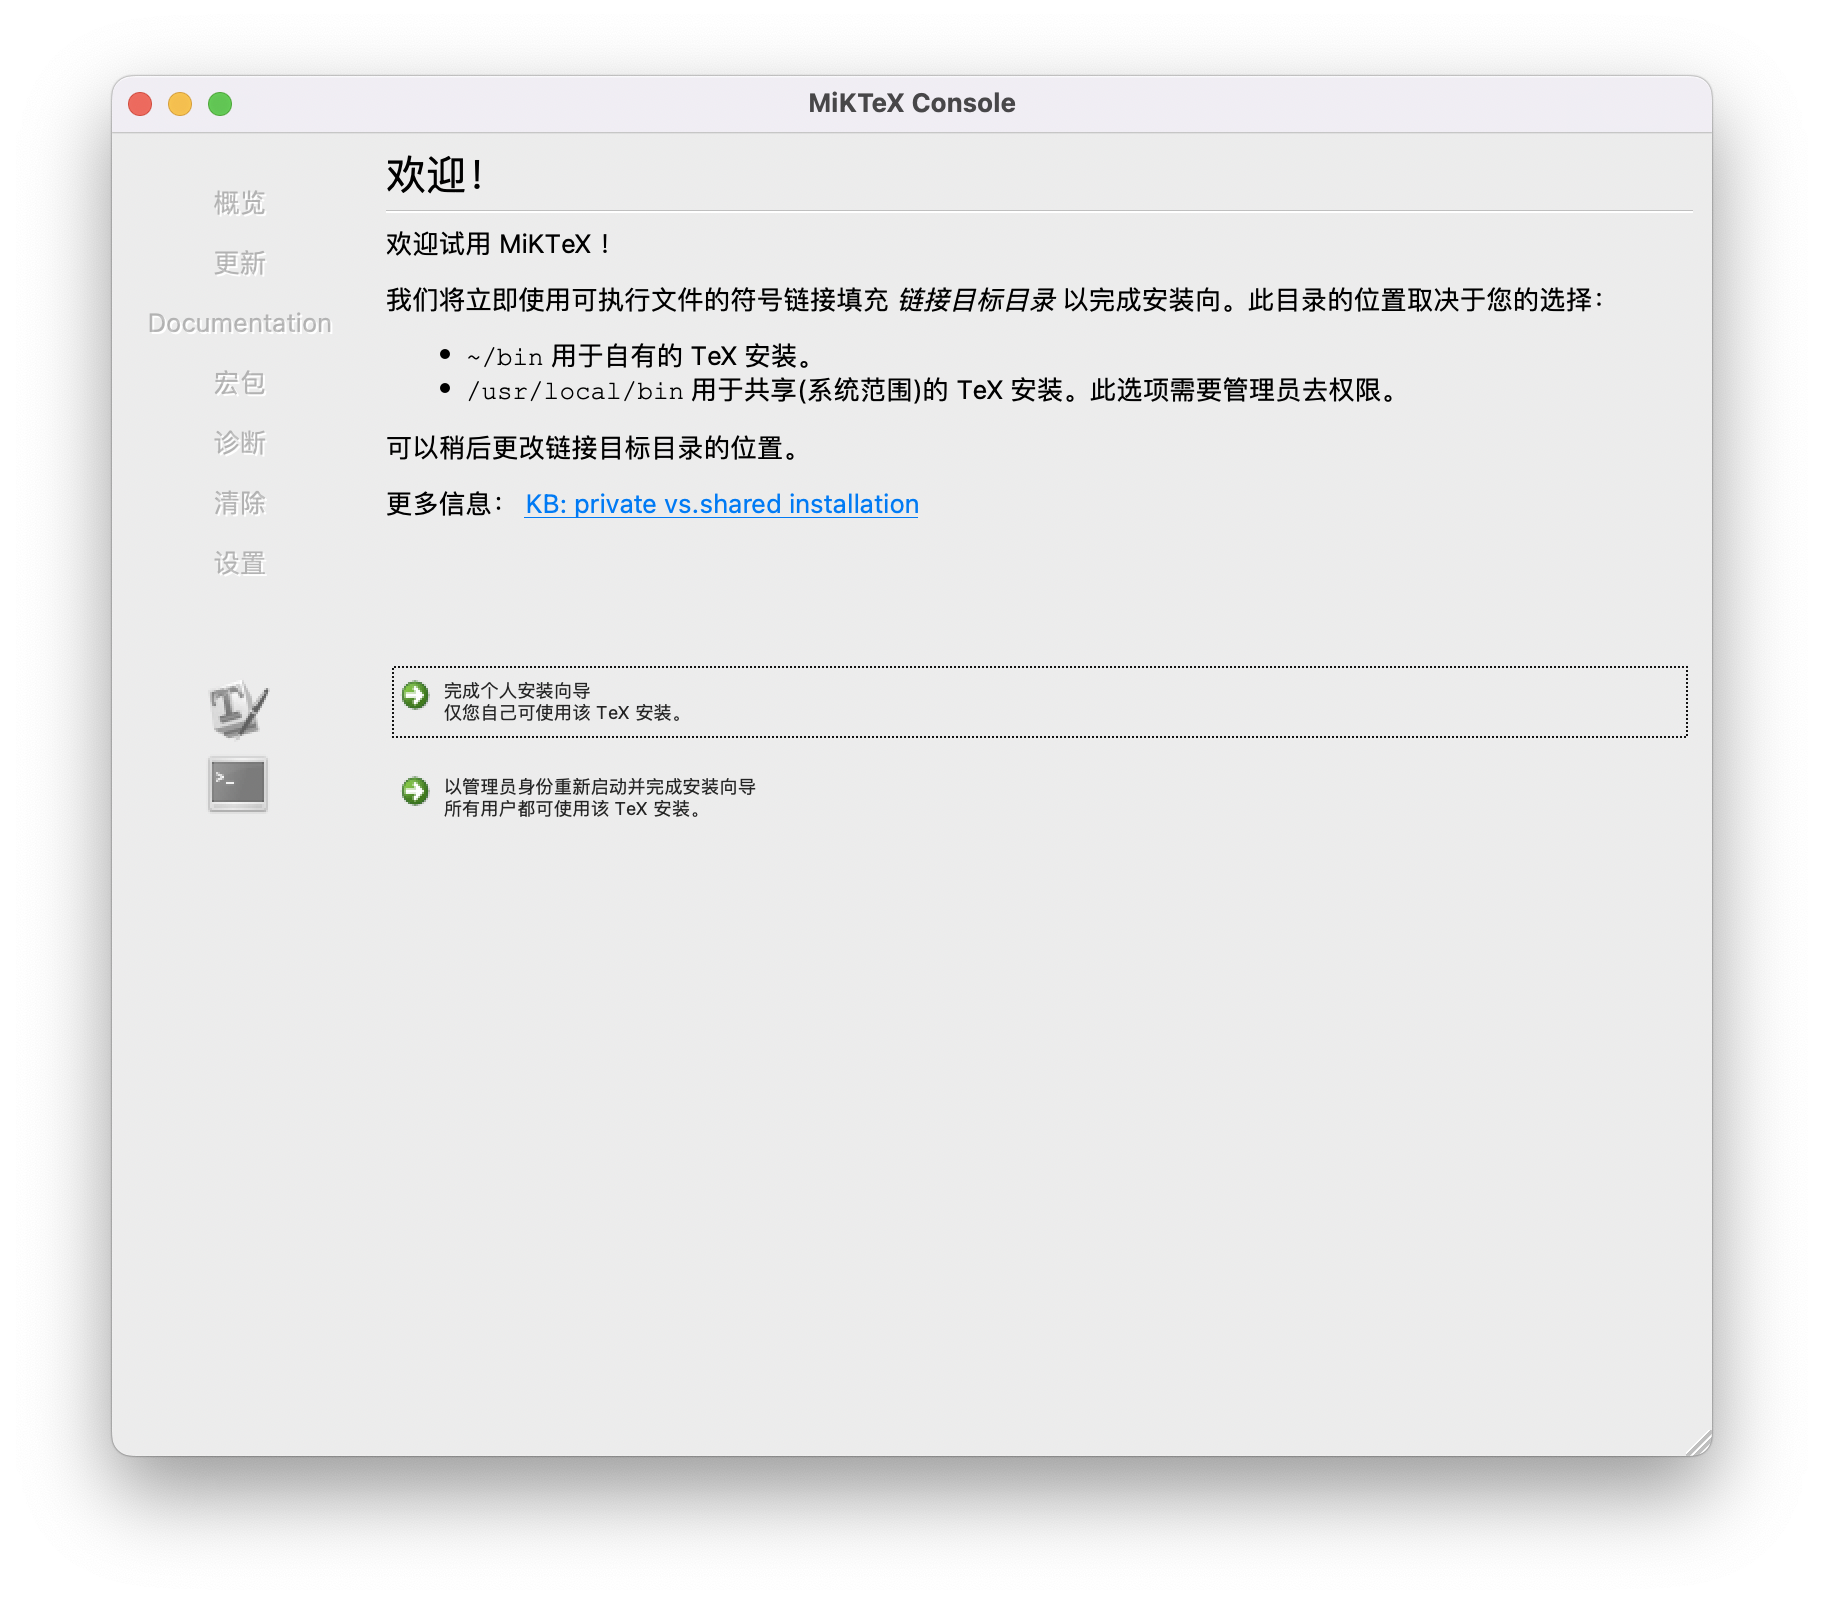
\includegraphics[width=0.9\textwidth]{miktex-console-mac}
\end{figure}

随后的设置方法与 Windows 系统下相同。从左侧栏切换到“更新”选项卡,点击“检查更新”按钮,待列表刷新后,点击“立即更新”按钮。

\begin{widepar}
更新完成后可以关闭 MiKTeX Console 应用程序,接着阅读 \ref{sec:hw}。
\end{widepar}

\subsection{Linux}
\label{subsec:mik-linux}

\begin{widepar}
你已经是一个成熟的 Linux 用户啦,乖乖去读\href{https://miktex.org/howto/install-miktex-unx}{官方文档}吧!
\end{widepar}
